\chapter{The Complex Numbers}

This text is entirely based around the study of $\C$, the set of complex numbers. How do complex functions behave? Can we differentiate and integrate? How does this differ from working over $\R$? In due time, we will see all of this. But before we can get to any of that, we need to discuss what $\C$ is and how to do algebra in the complex numbers.

\section{What is $\C$?}

\begin{defbo}{The Complex Numbers}{complexNumbers}
The imaginary unit $i$ is a number such that $i^2 = -1$. A complex number is a number of the form $a + bi$, where $a,b\in \R$. The set of complex numbers is $\C = \{a + bi| a,b\in \R\}$.
\end{defbo}

\begin{note}The name "imaginary" is a misnomer. When mathematicians first started thinking about complex numbers, $i$ was treated at best as a calculation trick and at worst as pure nonsense. The name was originally chosen as an insult.

Now, we recognize that the concept is real in the same way any other advanced mathematics is. These actually exist, and we can formally design a system that exhibits this behavior.

Beyond that, however, complex numbers are actually useful in real life. For example, the mathematics behind electomagnetism is based on working with complex numbers.\end{note}

\begin{ex}{}{} For example, $2 + 3i$, $\pi - ie^2$, and $1$ are all complex numbers.

Why would $1$ be a complex number? Isn't it real? When we write $1$ in this context, we mean $1 + 0i$. In this way, we can think of every real number $r$ as a complex number as well: $r = r + 0i$.
\end{ex}

\section{Complex Algebra}

Let's talk about how to manipulate complex numbers. Our overarching goal is to develop some notion of calculus. This requires us to be able to do algebra on $\C$.

\begin{defbo}{Real and Imaginary Parts}{ReAndIm}\index{Algebra!real part}\index{Algebra!imaginary part} 
Let $a+ bi\in \C$. Then the {\bf real and imaginary parts} of $a+bi$ are:

$$\RE(a+bi) = a$$
$$\IM(a+bi) = b$$
\end{defbo}

\begin{ex}{}{} Consider $z = 3 + 4i$. The real part of $z$ is $3$, and the imaginary part is $4$. Notice: $4$, not $4i$. The imaginary part of $z$ is still a real number.
\end{ex}


\begin{defbo}{Addition}{addition}\index{Algebra!addition}
 Let $a+bi, c+di \in \C$. Then:

$$(a+bi) + (c+di) = (a+c) + (b+d)i$$
\end{defbo}

So adding $z,w \in \C$ is done by adding together the real parts of $z,w$, and adding together the imaginary parts.

\begin{defbo}{Multiplication}{multiplication}\index{Algebra!multiplication} 
Let $a + bi, c+di \in \C$. Then:

$$(a+bi)(c+di) = ac - bd + (ad + bc)i$$
\end{defbo}

Why would we choose this definition? Well, we want complex multiplication to satisfy the "distributivity property": $(a+b)c = ac+bc$ and $a(b+c) = ab + ac$. If we require these to hold, then we are forced to conclude that:

\begin{align*}(a+bi)(c+di) &= (a+bi)c + (a+bi)di\\
&= (ac + bic) + (adi + bidi)\\
&= ac + bci + adi + bdi^2\\
&= ac + bci + adi - bd\\
&= (ac -bd) + (ad + bc)i
\end{align*}

Complex multiplication and addition satisfy a whole bunch of properties, specifically what are called the field axioms.


\begin{thmbo}{The Field Axioms}{fieldAxioms}
The complex numbers satisfy the following properties. For all $u, w, z \in \C$:

\begin{enumerate}
\item  $w + z = z + w$
\item  $u + (w + z) = (u+ w) + z$
\item  $z + 0 = z$
\item If $z = x + iy$, then $-z = (-x) + i(-y)$ satisfies that $z + (-z) = 0$.
\item $wz = zw$
\item $u(wz) = (uw)z$
\item $1z = z$
\item For any $z\in \C$ with $z\ne 0 + 0i$, there exists some $w\in \C$ with $zw = 1$. 
\item $u(w+z) = uw + uz$ and $(u+w)z= uz + wz$
\end{enumerate}
\end{thmbo}

\begin{proof} Many of these properties aren't hard to check, and follow pretty quickly from facts you know about real numbers.

We will provide a proof for the existence of multiplicative inverses very shortly, before we discuss division. \end{proof}

\begin{ex}{}{} Let $z = 2 + 7i$, $w = 4 - 3i$. Find $w^2 - zw$.

Well, to make life simpler, we can factor (using distributivity):
$$w^2 - zw = w(w-z) = (4-3i)[(4-3i) - (2 + 7i)] = (4-3i)(2 - 10i) = (8 - 30) + (-40 - 6)i = -22 - 46i$$

\end{ex}

What about division? First, what is division? What does $\frac{1}{z}$ mean? 

\begin{defbo}{Multiplicative Inverse}{multinv}
Let $z\in \C$. We say that $w = \frac{1}{z}$ if $zw =1$. In this situation, $w$ is a {\bf multiplicative inverse} for $z$. The existence of such a $w$ is one of the field axioms.
\end{defbo}

So how do we find a multiplicative inverse for $z$? To do that, we're going to need to introduce two new ideas, the complex conjugate and the modulus:

\begin{defbo}{Complex Conjugate}{conjugate}\index{Algebra!complex conjugate} 
Let $a+bi \in \C$. Then the {\bf complex conjugate} of $a+bi$ is:

$$\overline{a+bi} = a-bi$$
\end{defbo}

\begin{defbo}{Modulus}{modulus}\index{Algebra!modulus} 
Let $a+bi \in \C$. Then the {\bf modulus} of $a+bi$ is the real number:

$$|a+bi| = \sqrt{a^2 + b^2}$$
\end{defbo}

How does this help us define division? It turns out, these are exactly the building blocks we need:

\begin{lem}Let $a+bi\in \C$ be non-zero (i.e., at least one of $a,b$ is not 0). Then $\frac{1}{z} = \frac{a}{a^2 + b^2} - \frac{b}{a^2 + b^2}i$. Another way of writing this is that $\frac{1}{z} = \frac{\overline{z}}{\left|z\right|^2}$, where we understand that division by a real number means division on both the real part and imaginary part.\end{lem}

\begin{proof} To show that $\frac{1}{z}$ is what we claim, we need only check that $z\frac{1}{z} = 1$. We compute:

\begin{align*}(a+bi)\left(\frac{a}{a^2 + b^2} - \frac{b}{a^2 + b^2}i\right) &= \frac{a^2 -(b)(-b)}{a^2 + b^2} + \frac{ab + a(-b)}{a^2 + b^2}i\\
&= \frac{a^2 + b^2}{a^2 + b^2}\\
&= 1\end{align*}

\end{proof}

Where did this come from? The intuition comes from the calculation:

$$\frac{1}{a+bi}{\frac{a-bi}{a-bi}} = \frac{a-bi}{(a-bi)(a+bi)} = \frac{a-bi}{a^2 + b^2}$$

We can't use this as a proof of the result, since it relies on being able to divide by complex numbers (which we haven't even defined yet!), as well as being able to manipulate fractions. However, as far as intuition goes, this is a good way to understand the result.

\begin{note} This calculation also shows that $z\OL{z} = |z|^2$. This is a very important fact, and will come up very frequently.\end{note}


This lemma lets us define division properly:

\begin{defbo}{Division}{division}\index{Algebra!division} 
Let $z,w\in \C$ with $w\ne 0$. Then:
$$\frac{z}{w} = \frac{z\overline{w}}{|w|^2}$$
\end{defbo}


\begin{ex}{}{} Let $z = 4 + 3i$ and $w = 1 + i$. Find $\frac{z}{w}$ and $\frac{w}{z}$.

We know from our formula that $\frac{z}{w} = \frac{z\overline{w}}{|w|^2}$. So we compute:
$$\overline{w} = 1 - i$$
$$|w|^2 = (1^2 + 1^2)  = 2$$
So, $\frac{z}{w} = \frac{(4 + 3i)(1 - i)}{2} = \frac{7}{2} -\frac{1}{2}i$.


To compute $\frac{w}{z}$, we could go through the same process. Or, we could note that $\frac{w}{z} = \frac{1}{\left(\frac{z}{w}\right)} = \frac{2}{7 - i}$. We then get that:

$$\frac{w}{z} = \frac{2(7+i)}{|7-i|^2} = \frac{14}{50} + \frac{2}{50}i$$

\end{ex}

How do complex conjugation and the modulus behave when combined with our algebraic operations?

\begin{thmbo}{Algebraic Properties of Conjugation and the Modulus}{conjprop}Let $z,w \in \C$.

\begin{enumerate}
\item $\OL{zw} = \OL{z}\,\OL{w}$
\item $\OL{z + w} = \OL{z} + \OL{w}$
\item $\OL{\OL{z}} = z$.
\item $z + \OL{z} = 2\RE(z)$ and $z - \OL{z} = 2\IM(z)i$.
\item $\OL{\left(\frac{z}{w}\right)} = \frac{\OL{z}}{\OL{w}}$
\item $|zw| = |z||w|$
\item $|\OL{z}| = |z|$
\item If $z = x + iy$, then $|x| \le |z|$ and $|y| \le |z|$.
\item The {\bf triangle inequality}: $|z + w| \le |z| + |w|$. And $|z + w| = |z| + |w|$ if and only if $z = rw$ for some $r\in [0,\infty)$ or $w = rz$ for some $r\in [0,\infty)$.
\item $\left|\frac{z}{w}\right| = \frac{|z|}{|w|}$
\end{enumerate}

\end{thmbo}

\begin{proof} We will prove some, but not all of these statements. Many of them are variations on the same idea, and so will be quick to verify.

Let $z = a+ bi$ and $w = c + di$.

\begin{enumerate}
\item From the definition, $zw = ac -bd + (ad + bc)i$. Therefore, 

$$\OL{zw} = (ac - bd) - (ad + bc)i$$

On the other hand, we find that:

$$\OL{z}\,\OL{w} = (a-bi)(c-di) = (ac - (-b)(-d)) + (a(-d) + (-b)c)i = (ac - bd) - (ad +bc)i$$

So we see that $\OL{zw} = \OL{z}\,\OL{w}$.

\setcounter{enumi}{3}

\item We have $z + \OL{z} = a + bi + (a-bi) = 2a = 2\RE(z)$, and $z - \OL{z} = (a + bi) - (a-bi) = 2bi = 2\IM(z)i$.

\setcounter{enumi}{7}

\item  Note that $|x| = \sqrt{x^2} \le \sqrt{x^2 + y^2}$, since $f(x) =\sqrt{x}$ is an increasing function on $[0,\infty)$ and $y^2\ge 0$. This shows that $|x| \le |z|$. A similar argument shows that $|y| \le |z|$.

\item To show this, it is enough to show that $|z+w|^2 \le (|z| + |w|)^2$. It will take us a bit of work to get there though.

%
%
%First, note that $(|z| + |w|)^2 = |z|^2 + 2|z||w| + |w|^2 = $. 
%
%On the other hand:
%
%\begin{align*}|z + w|^2 &= (z + w)(\OL{z} + \OL{w}) \\
%&= z\OL{z} + (z\OL{w} + \OL{z}w) + w\OL{w} \\
%&= |z|^2 + (z\OL{w} + \OL{z\OL{w}}) + |w|^2\\
%&= |z|^2 + 2\RE(z\OL{w}) + |w|^2
%\end{align*}
%
%So, we have $|z +w|^2 = |z|^2 + 2\RE(z\OL{w}) + |w|^2 \le |z|^2 + 2|z\OL{w}| + |w|^2= |z|^2 + 2|z||w| + |w|^2 = (|z| + |w|)^2$. Taking square roots of both sides gives the desired inequality.
%
%From this calculation, notice that $|z + w| = |z| + |w|$ if and only if $2\RE(z\OL{w}) = 2|z||w|$. Therefore, this occurs precisely when $ac + bd = \sqrt{a^2 + b^2}\sqrt{c^2 + d^2}$.
%
%
%
%
%
%
%


First, notice that $(ad - bc)^2 \ge 0$. This implies that

$$2abcd \le a^2d^2 + b^2c^2$$

Adding $a^2c^2 + b^2d^2$ to both sides tells us that:

$$(ac + bd)^2 \le (a^2 + b^2)(c^2 + d^2)$$

As such, it follows that $2(ac + bd) \le 2\sqrt{(a^2 + b^2)(c^2 + d^2)}$. Now, adding $a^2 + b^2 + c^2 + d^2$ to both sides gives:

$$(a^2 + 2ac + c^2) + (b^2 + 2bd + d^2) \le (a^2 + b^2) + 2\sqrt{(a^2 + b^2)(c^2 + d^2)} + (c^2 + d^2)$$

Factoring each side gives:

$$(a+c)^2 + (b+d)^2 \le (\sqrt{a^2 + b^2} + \sqrt{c^2 + d^2})^2$$

However, $(a+c)^2 + (b+d)^2 = |z+w|^2$, $\sqrt{a^2 + b^2}= |z|$, and $\sqrt{c^2 + d^2} = |w|$. So we have shown that $|z+w|^2 \le (|z|  +|w|)^2$. Taking the square root of both sides gives $|z +w| \le |z| + |w|$.


For equality, assume WLOG that $z = rw$ for some $r\in [0,\infty)$ (you should consider how the modify this in the case where $w = rz$), then $c = ar$ and $b = dr$ so $ad - bc = 0$. In that case:

$$2abcd = a^2d^2 + b^2c^2$$

Following the same steps as above, we find that $ac+bd) = r(a^2+b^2) > 0$. So $\sqrt{(ac+bd)^2} = ac+bd$. So we have $2(ac+bd) = 2\sqrt{(a^2+b^2)(c^2+d^2)}$. Continuing the computation gives the desired result.

Suppose instead that $|z+w| = |z| + |w|$. Then we must have that $ac +bd = \sqrt{(a^2+b^2)(c^2+d^2)}$. Working backwards along our computation above, we see that this means we must have $ad - bc = 0$. From linear algebra, this gives that $\{(a,b),(c,d)\}$ is a linearly dependent set and so there exists $r\in \R$ such that either $z = rw$ or $w = rz$. Furthermore, since $\sqrt{(a^2+b^2)(c^2+d^2)} \ge 0$, we must have $ac + bd > 0$. Since $ac+bd = r(a^2+b^2)$ or $r(c^2+d^2)$, we see that we must also have $r \ge 0$ as desired.

\begin{note}Fisher has a shorter proof of this fact in section 1.2. However, he does not discuss equality.\end{note}


\item To begin, let's show that $\left|\frac{1}{w}\right| = \frac{1}{|w|}$. Notice that $\frac{1}{w} = \frac{c}{c^2 + d^2} - \frac{d}{c^2 + d^2}i$. And so:

\begin{align*}\left|\frac{1}{w}\right| &= \sqrt{\left(\frac{c^2}{(c^2 + d^2)^2} + \frac{d^2}{(c^2 + d^2)^2}\right)} \\
&= \sqrt{\frac{1}{c^2 + d^2}}\\
&= \frac{1}{\sqrt{c^2 + d^2}}\\
&= \frac{1}{|w|}
\end{align*}

Now, by the first result of this theorem, we see that:

$$\left|\frac{z}{w}\right| = |z|\left|\frac{1}{w}\right| = |z|\frac{1}{|w|} = \frac{|z|}{|w|}$$

\end{enumerate}

\end{proof}


\section{Rectangular Coordinates and $\R^2$}

One way of visualizing complex numbers is to picture them as a vector in $\R^2$.

\begin{ex}{}{} Consider $z = 3 + 2i$. Then we can visualize $z$ as the vector:

\begin{center}
\begin{tikzpicture}
%\draw [help lines,black!20!white] (-1,-1) grid (4,4);
\foreach \x in {-1,1,2,3}
       \draw[xshift=\x cm, thick] (0pt,-1pt)--(0pt,1pt) node[below] {$\x$};
\foreach \y in {-1,1,2,3}
       \draw[yshift=\y cm, thick] (-1pt,0pt)--(1pt,0pt) node[left] {$\y$};    

\draw[thick] (0,-1) -- (0,3);
\draw[thick] (-1,0) -- (3,0);

\draw[->] (0,0) -- (3,2);

\draw (3,2) node[above]{$z$}; 

\end{tikzpicture}
\end{center}

\end{ex}

\begin{note} In general, we can visualize the complex number $z = x + iy$ as the point $(x,y)$ on the plane.

However, this does not mean that $\C$ and $\R^2$ are the same thing. They are not. We cannot multiply vectors in $\R^2$. We can't divide by vectors. Etc.
\end{note}

\begin{defbo}{Rectangular Coordinates}{rectCoords} \index{Coordinates!rectangular} The {\bf rectangular coordinates} of $z \in \C$ is the point $(\RE(z), \IM(z))$ in $\R^2$.

When we write $z = x + iy$, we say that $z$ is written in {\bf rectangular form}.
\end{defbo}


This perspective does allow us to give some fairly nice proofs. For example:

\begin{thmbo}{The Triangle Inequality}{triangIneq}
 Let $z = x+iy$. Then $|z|$ is equal to the length of the vector $(x,y)$.

\vspace{5pt}

As a consequence, $|z + w| \le |z| + |w|$.
\end{thmbo}

\begin{proof} The first claim is fairly straightforward: $|z| = \sqrt{x^2 + y^2}$, and the length of the vector $(x,y)$ is $\lVert (x,y) \rVert = \sqrt{x^2 + y^2}$.

So, let $w,z\in \C$ and let $\vec{w}$ and $\vec{z}$ be their corresponding vectors in $\R^2$. Now, consider the following picture:

\begin{center}
\begin{tikzpicture}

\draw[thick] (0,-2) -- (0,3);
\draw[thick] (-2,0) -- (3,0);


\node at (0,0) (origin){};
\node at (1,2) (z){};
\node at (2,-1) (sum){};

\draw[->] (origin) -- (z) node [midway, left]{$\vec{z}$};

\draw[->, red] (z)-- (sum) node [midway, right]{$\vec{w}$};

\draw[->, blue] (origin) -- (sum) node [inner sep = 9pt, midway, below]{$\vec{z} + \vec{w}$};

\end{tikzpicture}
\end{center}

The vectors $\vec{z}$,  $\vec{w}$, and $\vec{z} + \vec{w}$ satisfy the triangle inequality: $\lVert \vec{z} + \vec{w} \rVert \le \lVert\vec{z}\rVert + \lVert\vec{w}\rVert$. And further, equality occurs precisely when $\vec{z}$ and $\vec{w}$ are in the same direction.

However, since the lengths of these vectors are equal to the corresponding moduli of the complex numbers, we conclude the triangle inequality on $\C$.

\end{proof}

\section{Polar Coordinates}

Let $z = x + iy$. We have seen that there is one way to represent complex numbers visually, via rectangular coordinates. There is another, which is in many ways much more important. Consider the picture:

\begin{center}
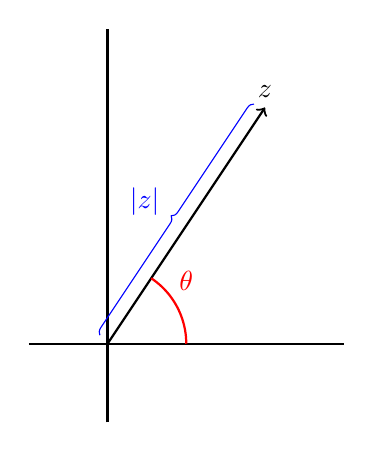
\begin{tikzpicture}
%\draw [help lines,black!20!white] (-1,-1) grid (4,4);

\draw[thick] (0,-1) -- (0,4);
\draw[thick] (-1,0) -- (3,0);

\draw[thick, ->] (0,0) -- (1.2,1.8) node [blue, inner sep = 15pt, left]{$|z|$} -- (2,3);
\draw[blue, decorate, decoration = {brace, raise = 4pt}] (0.02,0.03)--(1.98,2.97);

\draw (2,3) node[above]{$z$}; 

\draw [red,thick,domain=0:56.3] plot ({cos(\x)}, {sin(\x)});

\draw (1, 0.8) node [red] {$\theta$};

\end{tikzpicture}
\end{center}

We can also express this vector in $\R^2$ by giving its length, $|z|$, and the angle it forms with the positive $x$-axis, $\theta$.

\begin{lem} If $z\in \C$ with $|z| = r$, and $z$ forms an angle of $\theta$ with the positive $x$-axis, then:

$$z = r(\cos(\theta) + i\sin(\theta))$$
\end{lem}

\begin{proof} Suppose $|z| = r$. Then the vector $\vec{z}$ in $\R^2$ has $\lVert \vec{z}\rVert = r$. As such, $\vec{z}$ is on a circle of radius $r$, which we know (from MAT235) is parametrized by the equations $x = r\cos(\theta)$ and $y = r\sin(\theta)$, where $\theta$ is the angle between $\vec{z}$ and the positive $x$-axis.

As such, we conclude that $z = x + iy = (r\cos(\theta)) + (r\sin(\theta))i$, as desired.
\end{proof}


\begin{defbo}{Polar Coordinates}{polarCoords}\index{Coordinates!polar}
 Let $z\in \C$. Then we say that $z$ is in {\bf polar coordinates}, or in {\bf polar form}, if we write $z$ as $z = r(\cos(\theta) + i\sin(\theta))$.

In this expression, $r = |z|$ and $\theta$ is the angle between $z$ and the positive $x$-axis.
\end{defbo}

\begin{ex}{}{} Find the real and imaginary parts of $z = 2(\cos(0.2) + i\sin(0.2))$.

Well, $z = 2\cos(0.2) + (2\sin(0.2))i$, and so $\RE(z) = 2\cos(0.2)$ and $\IM(z) = 2\sin(0.2)$.

\end{ex}

\begin{note} Be careful! The real part of $z$ is not $2$. $2$ is its modulus! This is a very common mistake!\end{note}


\begin{ex}{}{} Write $z = 4 - 4\sqrt{3}i$ in polar form.

Let's start by finding $|z|$. This is always easier. We compute: $|z| = \sqrt{16 + (16)(3)} = \sqrt{64} = 8$.

Now, we can see that $z$ forms a right angle triangle with the positive real axis which has hypotenus $8$, and side lengths $4$ and $4\sqrt{3}$. If we view this as:

\begin{center}
\begin{tikzpicture}
%\draw [help lines,black!20!white] (-1,-1) grid (4,4);

\draw[thick] (0,-4) -- (0,1);
\draw[thick] (-1,0) -- (3,0);

\draw[->] (0,0) -- (2,-3);

\draw (2,-3) node[below]{$z$}; 

\draw [red,thick,domain=0:-56.3] plot ({cos(\x)}, {sin(\x)});

\draw (1, -0.8) node {$\Psi$};

\end{tikzpicture}
\end{center}

Then we have that $\Psi = -\theta$ and that:
\begin{align*} \cos\Psi &= \frac{4}{8} = \frac{1}{2}\\
\sin(\Psi) &= \frac{4\sqrt{3}}{8} = \frac{\sqrt{3}}{2}
\end{align*}

We know from our special triangles that this gives $\Psi = \frac{\pi}{3}$. Therefore, $\theta = -\frac{\pi}{3}$.

So, in polar form, we have $4 - 4\sqrt{3}i = 8\left(\cos\left(\frac{-\pi}{3}\right) + i\sin\left(\frac{-\pi}{3}\right)\right)$.

\end{ex}

There is another bit of notation, which you may have come across, used to write polar form.

\begin{defbo}{Euler's Formula}{eulerForm}\index{Euler's Formula} 
$e^{i\theta} = \cos(\theta) + i\sin(\theta)$.
\end{defbo}

So, instead of writing $z = r(\cos(\theta) + i\sin(\theta))$, we will from now on write $z = re^{i\theta}$. We will discuss why we use this notation (why $e$?), later on in the course. There is a reason.

\begin{ex}{}{} Find the polar form for $z = \frac{-1}{\sqrt{2}} + \frac{1}{\sqrt{2}}i$, and write it as $z = re^{i\theta}$.

We know that $r = |z|$. So we compute:
$$|z| = \sqrt{\left(\frac{-1}{\sqrt{2}}\right)^2 + \left(\frac{1}{\sqrt{2}}\right)^2} = \sqrt{1} = 1$$

As for the angle, we need to be careful here. If we were to take the angle $\theta = \arctan\left(\frac{y}{x}\right) = \arctan(-1)$, we would end up with an angle in the fourth quadrant. But our complex number is in the second quadrant. So how do we handle this?

Well, note that our angle $\theta$ and $\arctan(-1)$ are on directly opposite sides of the unit circle, and so $\theta = \arctan(-1) + \pi = \frac{3 \pi}{4}$.

Therefore, $z = 1e^{i\frac{3\pi}{4}}$.

\end{ex}

\begin{ex}{}{} True or false: the real part of $3e^{i\frac{\pi}{2}}$ is $3$.

False. This is a mistake I have seen quite a lot. You need to be able to find the real and imaginary parts of a complex number written in polar form.

In this case, $3e^{i\frac{\pi}{2}} = 3\left(\cos\left(\frac{\pi}{2}\right) + i\sin\left(\frac{\pi}{2}\right)\right) = 3(0 + i) = 3i$. So the real part of this complex number is 0!

\end{ex}

Polar coordinates are useful in a variety of ways, which are majorly different from the ways in which rectangular form is useful. One way is that working in polar form makes doing multiplication very easy.

\begin{thmbo}{Multiplication in Polar Form}{polarmult} \index{Algebra!multiplication in polar form}
 Let $z = re^{i\theta}$ and $w = Re^{i\Psi}$. Then:
$$zw = rRe^{i(\theta + \Psi)}$$
\end{thmbo}

\begin{proof} We go back to rectangular coordinates. $z = r(\cos(\theta) + i\sin(\theta))$ and $w = R(\cos(\Psi) + i\sin(\Psi))$. Then:

\begin{align*} zw =& rR(\cos(\theta) + i\sin(\theta))(\cos(\Psi) + i\sin(\Psi))\\
=& rR\left(\left[\cos(\theta)\cos(\Psi) - \sin(\theta)\sin(\Psi)\right]\right.\\
& +\left. i\left[\sin(\theta)\cos(\Psi) + \cos(\theta)\sin(\Psi)\right]\right)\\
=&rR(\cos(\theta + \Psi) + i\sin(\theta + \Psi) \qquad\qquad (\text{trig identities})\\
=&rRe^{i(\theta + \Psi)}
\end{align*}

\end{proof}

A similar argument can also be used to prove: 

\begin{thmbo}{Division in Polar Form}{polarDiv} \index{Algebra!division in polar form}
 Let $z = re^{i\theta}$ and $w = Re^{i\Psi}\ne 0$. Then:
$$\frac{z}{w} = \frac{r}{R}e^{i(\theta - \Psi)}$$
\end{thmbo}

\begin{proof} The proof is similar to that of theorem \ref{thm:polarmult}, except using the angle difference formulas for $\sin$ and $\cos$. Consider working through the proof, mimicing the proof of theorem \ref{thm:polarmult}.\end{proof}

\begin{note} The key ingredients in these proofs are trig identities. Specifically, the angle sum (and angle difference) formulas. Trig is very important to working with complex numers. You will need to know your trig identities. \end{note}


Since multiplying in polar form is very quick, taking powers should also be really quick. Intuitively, the argument above tells us that if $\theta$ is an angle for $z$, then $n\theta$ is an angle for $z^n$. After all, if we add $n$ copies of $\theta$, we get $n\theta$. This intuitive idea is actually a named theorem!

\begin{thmbo}{De Moivre's Theorem}{demoivre} \index{De Moivre's Theorem}
Let $n\in \N$. Then $(\cos(\theta) + i\sin(\theta))^n = \cos(n\theta) + i\sin(n\theta)$.
\end{thmbo}

\begin{proof} We proceed by induction. The claim is clearly true for $n = 1$.

Suppose $(\cos(\theta) + i\sin(\theta))^n = \cos(n\theta) + i\sin(n\theta)$. This really just says: $(e^{i\theta})^n = e^{i(n\theta)}$.

Now, consider $(\cos(\theta) + i\sin(\theta))^{n+1}$. We have:

\begin{align*} (\cos(\theta) + i\sin(\theta))^{n+1} &= (e^{i\theta})^{n+1}\\
&= (e^{i\theta})^ne^{i\theta}\\
&= e^{i(n\theta)}e^{i\theta} \qquad\qquad\qquad\qquad \qquad   (\text{by the induction hypothesis})\\
&= e^{i(n+1)\theta} \qquad \qquad\qquad \qquad\qquad 	 	 (\text{by theorem \ref{thm:polarmult}})\\
&= \cos((n+1)\theta) + i\sin((n+1)\theta)
\end{align*}
\end{proof}


We end our discussion of complex algebra with one last definition. We will need to talk about the polar form, and specifically the angle, of a complex number very often.

\begin{defbo}{The Argument}{argument}\index{Argument} Let $z = re^{i\theta}$ be non-zero. The angle $\theta$ is called an argument for $z$.

We do not define an argument for $z = 0$.
\end{defbo}

The argument of a complex number is not unique. For example, $e^{i0} = 1$, and $e^{i2\pi} = \cos(2\pi) + i\sin(2\pi) = 1$. This means that $0$ and $2\pi$ are both arguments for $1$!

\begin{ex}{}{} Is $\frac{7\pi}{3}$ an argument for $1 + \sqrt{3}i$?

There are two approaches to this. One way would be to find an argument for $1 + \sqrt{3}i$. We recognize this as appearing on a 30-60-90 special triangle of hypotenuse 2, in the first quadrant. In particular, $\theta = \frac{\pi}{3}$ is an argument for $1 + \sqrt{3}i$.

Then we quickly check that $\frac{\pi}{3}$ and $\frac{7\pi}{3}$ point in the same direction, since they differ by a multiple of $2\pi$.

\vspace{10pt}

Another approach would be to see what $e^{i\frac{7\pi}{3}}$ is. We find that $e^{i\frac{7\pi}{3}} = \frac{1}{2} + \frac{\sqrt{3}}{2}i$, and so $1 + \sqrt{3}i = 2e^{i\frac{7\pi}{3}}$. So $\frac{7\pi}{3}$ is an argument for $1 + \sqrt{3}$.

\end{ex}

The non-uniqueness of the argument ends up giving the complex numbers a lot of rich theory. For example, every non-zero number will have $n$ different $n^{\text{th}}$ roots. Every complex number will have infinitely many logarithms. We'll see this when we talk about the concept of ``branches".

Sometimes, we don't need all that freedom. Very often, it's enough to consider arguments within a specific range. One particular choice is $(-\pi,\pi)$.

\begin{defbo}{The Principal Argument}{principalArg}\index{Argument!principal}\index{Argument!$\Arg(z)$}
Let $z\in \C$ such that $z$ is not a negative real number. The principal arugment of $z$ is the argument $\Arg(z) \in (-\pi,\pi)$.
\end{defbo}

\begin{note} This is a different covention that some other sources you may encounter. I am specifically excluding negative reals from having a principal argument. I am not doing this arbitrarily however: this will allow us to avoid some ugly continuity issues later on when we define the principal logarithm, or other principal branches of multivalued functions.\end{note}


\section{$n^{\text{th}}$ roots}

We now turn our attention to square and higher roots. What is an $n^{\text{th}}$ root, and how do we find them?

\begin{defbo}{$n^{\text{th}}$ Roots}{roots}
Let $n\in\N$. Then we say that $z$ is an $n^{\text{th}}$ root of $w$ if $z^n = w$.
\end{defbo}

In the real numbers, solving the equation $x^n = c$ is fairly straightforward. If $n$ is even, then it has no solution for $c < 0$. And for $c \ge 0$, the solutions are $x = \pm\sqrt[n]{c}$. For $n$ odd, there is always a unique solution: $x = \sqrt[n]{c}$.

We have already seen that this is no longer true for complex numbers. In particular, the equation $z^2 = -1$ has a solution: $i$ (and $-i$ as well). This is true in a much more broad sense. The equation $z^n = c$ always has a solution, and De Moivre's theorem tells us exactly how to find such solutions.

Let us begin with an example, to see the general tactic in action.

\begin{ex}{}{} Find all square roots of $z^2 = 1 + i$.

There are a couple of ways to approach this. One way is to write $z = x + iy$, and then expand $z^2 = 1+i$ to get the equations:
$$x^2 - y^2 = 1$$
$$2xy = 1$$

Now, this is solvable. For example, we can write $y = \frac{1}{2x}$, and substitute this into the first equation, giving $x^2 - \frac{1}{4x^2} = 1$. Rearranging to give $4x^4 - 4x^2 - 1 = 0$. We can then use the quadratic formula to find $x$.

However, this approach has some major drawbacks. This isn't an easy calculation, to start. But worse, it doesn't generalize. For example, if we wanted to solve $z^3 = 1+i$, we would need to solve the system $x^3 - 3xy^2 = 1$ and $3x^2y - y^3 = 1$, which is quite a bit more difficult. This approach doesn't work for higher powers.

Instead, let's see what happens if we work in polar form. Let $z = re^{i\theta}$. Then we have:
$$r^2e^{2i\theta} = 1 + i = \sqrt{2}e^{i\frac{\pi}{4}}$$

By comparing moduli on both sides, we find $r^2 = \sqrt{2}$, so $r = \sqrt[4]{2}$.

Also, by comparing arguments, we see that $2\theta$ is an argument for $1 + i$. I.e., $2\theta = \frac{\pi}{4} + 2k\pi$ for some $k\in \Z$.

As such, $z = \sqrt[4]{2}e^{i\frac{\pi}{8} + k\pi}$ for some $k\in \Z$. Recalling that $e^{i\theta}$ is $2\pi$ periodic, we see that we only get two distinct solutions: $\pm\sqrt[4]{r}e^{i\frac{\pi}{8}}$. 
\end{ex}

Does this work generally? Is there some algorithm or formula that gives us $n^\text{th}$ roots?

\begin{thmbo}{Existence of $n^{\text{th}}$ Roots}{rootsExist}\index{Roots} 
Let $w = re^{i\theta} \in \C$. If $w = 0$, then $z^n = w$ has a unique solution, $z = 0$.

If $w\ne 0$, then the solutions to $z^n = w$ are:
$$z_j = \sqrt[n]{r}e^{\frac{i(\theta + 2j\pi)}{n}}$$

\noin where $j \in \Z$. Furthermore, it is enough to assume $j\in \{0,1,2,\dots,n-1\}$.
\end{thmbo}

\begin{proof} When $w = 0$, the claim is clear.

For $w\ne 0$, what do we need to show? We need:

\begin{itemize}
\item The $z_j$ are solutions to $z^n = w$. I.e., $z_j^n = w$.
\item The $z_j$ are the only solutions to $z^n = w$. I.e., if $z^n = w$, then $z = z_j$ for some $j$.
\end{itemize}

In other words, we need to prove that $z^n = w$ if and only if $z = z_j$ for some $j$. Let $z = se^{i\Psi}$ be in polar form. Then $z^n = w \iff  s^ne^{in\Psi} = re^{i\theta}$. This occurs if and only if $s^n = r$ and $n\Psi = \theta + 2k\pi$ for some $k\in \Z$, by considering the moduli and arguments of each side.

As such, $z^n = w$ if and only if $s = \sqrt[n]{r}$ and $\Psi = \frac{\theta + 2k\pi}{n}$ for some $k\in \Z$. I.e., $z^n = w$ if and only if $z = z_k$ for some $k\in \Z$.


Lastly, we need to justify why we only need to consider $j\in \{0,1,\dots,n-1\}$. Let $k\in \Z$. Then by the division algorithm, we can write $k = qn + j$ for some $0 \le j \le n-1$. We find that:

$$z_k = \sqrt[n]{r}e^{i\frac{\theta + 2k\pi}{n}} = \sqrt[n]{r}e^{i\frac{\theta + 2(qn + j)\pi}{n}} = \sqrt[n]{r}e^{i\frac{\theta+2j\pi}{n} + 2q\pi i} = \sqrt[n]{r}e^{i\frac{\theta + 2j\pi}{n}} = z_j$$

As such, each $z_k$ is actually equal to some $z_j$, where $0\le j \le n-1$.


Also, note that each of the $z_j$ for $j\in \{0,1,\dots,n-1\}$ are distinct. Since $\frac{\theta + 2j\pi}{n} \in \left[\frac{\theta}{n},\frac{\theta}{n} + 2\pi\right)$, we see that these angles all point in different directions.







%
%To begin, for $w\ne 0$, we should show that $z_j$ is a solution to $z^n = w$. I.e., we should show that $z_j^n = w$. However, we quickly see that 
%
%\begin{align*}z_j^n &= \left(\sqrt[n]{r}e^{\frac{i(\theta + 2j\pi)}{n}}\right)^n\\
%&= \sqrt[n]{r}^n \left(e^{\frac{i(\theta + 2j\pi)}{n}}\right)^n\\
%&= re^{\frac{in(\theta + 2j\pi)}{n}}\\
%&= re^{i(\theta + 2j\pi)} \\
%&= re^{i\theta}\\
%&= w\end{align*}
%
%Therefore, these $n$ distinct complex numbers are solutions to $z^n = w$. I leave it as an exercise for you to show they are distinct.
%
%
%Are these the only solutions?
%
%I have two arguments for you to show this.
%
%
%\paragraph{Polar form argument.} Suppose $z = |z|e^{i\Psi}$ satisfies that $z^n = w$. Then $w = z^n = |z|^ne^{in\Psi}$. However, we also know that $w = re^{i\theta}$.
%
%Now, since these complex numbers are equal, it must be that $r = |w| = |z^n| = |z|^n$, and so $|z| = \sqrt[n]{r}$.
%
%Furthermore, for these two complex numbers to be equal, they must be pointing in the same direction. I.e., $\theta$ and $n\Psi$ are arguments for the same complex number. This tells us that $n\Psi = \theta + 2k\pi$ for some $k\in \Z$. As such, $\Psi = \frac{\theta + 2k\pi}{n}$ for some $k\in \Z$.
%
%To see that we need only consider $j \in \{0,1,2,\dots, n-1\}$, note that for any $k\in \Z$, there exists $q,r\in \Z$ with $k = qn + r$ and $r\in \{0,1,2,\dots,n-1\}$, by division. Then $e^{i\frac{\theta + 2k\pi}{n}} = e^{i\left(\frac{\theta}{n} + \frac{2(qn+r)\pi}{n}\right)} = e^{i\left(\frac{\theta + 2r\pi}{n}\right) + i2q\pi} = e^{i\left(\frac{\theta + 2r\pi}{n}\right)}$. Therefore, each $k\in \Z$ yields the same root as one of the $z_j$.
%
%\paragraph{Algebra argument.} There is a much simpler argument, if we allow ourselves to stray a bit beyond the material of the course. Consider the polynomial $p(z) = z^n - w$. Over a field, a polynomial of degree $n$ has a most $n$ roots. However, we have shown that $p(z_j) = z_j^n -w = 0$ for $j = 0,1,2,\dots, n-1$. As such, we have given $n$ different roots for a degree $n$ polynomial. That must be all of the roots, and hence all the solutions to $z^n = w$.


\end{proof}

\begin{ex}{}{} Let $w = i$. Find all solutions to $z^2 = w$ and $z^4 = w$.


To begin, we need to write $w$ in polar form. In this case, it is simple: $w = e^{i\frac{\pi}{2}}$. The theorem gives us a formula for these roots.

To solve $z^2 = w$, we consider $z_0 = \sqrt{1}e^{i\frac{\pi/2}{2}} = e^{i\frac{\pi}{4}} = \frac{1}{\sqrt{2}} + \frac{i}{\sqrt{2}}$.

The other root is much easier to find. Notice that the other root is $z_1 = e^{i\frac{\pi/2 + 2\pi}{2}} = e^{i\frac{\pi/2}{2}}e^{\frac{2\pi}{2}} = -z_0$.

In solving $z^4 = w$, we can take a similar approach. Indeed, we have that $z_j = z_0e^{i\frac{2j\pi}{4}}$. This gives us a list:

\begin{itemize}
\item $z_0 = e^{i\frac{\pi}{8}}$
\item $z_1 = z_0e^{i\frac{2\pi}{4}} = iz_0$
\item $z_2 = z_0e^{i\frac{2*2\pi}{4}}= -z_0$
\item $z_3 = -iz_0$
\end{itemize}

As an interesting aside, it turns out that $e^{i\frac{\pi}{8}} = \frac{\sqrt{2 + \sqrt{2}}}{2} + i\frac{\sqrt{2 - \sqrt{2}}}{2}$. One possible way to show this would be to try to solve the equation $z^2 = \frac{1}{\sqrt{2}} + \frac{i}{\sqrt{2}}$ by setting $z = a + bi$.
\end{ex}

Notice, in our example, we factored $z_j$ as $\sqrt[n]{r}e^{i\frac{\theta}{n}}e^{i\frac{2j\pi}{n}}$. These numbers $e^{i\frac{2j\pi}{n}}$ are the $n^{\text{th}}$ roots of unity.

\begin{defbo}{Roots of Unity}{rootsUnity}\index{Roots!of unity}
The $n^{\text{th}}$ roots of unity are the solutions to $z^n = 1$. They are precisely the complex numbers $\omega_j = e^{i\frac{2j\pi}{n}}$.
\end{defbo}

\section{Geometry of roots}\index{Roots!geometry}

There are two nice geometric facts about the $n^{\text{th}}$ roots of $w$ that we can glean from the results of the previous section.

\begin{itemize}
\item Notice that $|z_j| = \sqrt[n]{r}$ for each $j$. This means that each of the $n^{\text{th}}$ roots of $w$ all lay on the circle of radius $\sqrt[n]{r}$ centered at $0$.

This circle has the equation $|z| = \sqrt[n]{r}$. More generally, a circle of radius $r$ centered at $z_0$ has the equation $|z-z_0| = r$. \index{Circle}

\item Notice that the angle between $z_j$ and $z_{j+1}$ is exactly $\frac{2\pi}{n}$.

So, for example, the $6$th roots of $w$ form a picture like:

\begin{center}
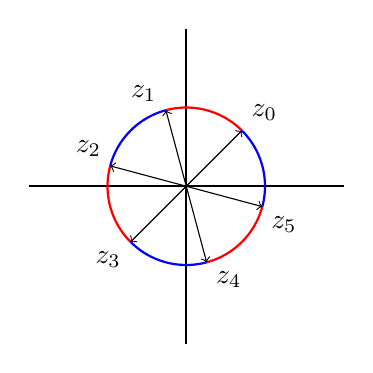
\begin{tikzpicture}
%\draw [help lines,black!20!white] (-1,-1) grid (4,4);

\draw[thick] (0,-2) -- (0,2);
\draw[thick] (-2,0) -- (2,0);


\draw [red,thick,domain= 45:105] plot ({cos(\x)}, {sin(\x)});
\draw [blue,thick,domain= 105:165] plot ({cos(\x)}, {sin(\x)});
\draw [red,thick,domain= 165:225] plot ({cos(\x)}, {sin(\x)});
\draw [blue,thick,domain= 225:285] plot ({cos(\x)}, {sin(\x)});
\draw [red,thick,domain= 285:345] plot ({cos(\x)}, {sin(\x)});
\draw [blue,thick,domain= 345:405] plot ({cos(\x)}, {sin(\x)});

\foreach \x in {0,1,...,5}
	\draw[->] (0,0) -- ({cos(45 + 60*\x)},{sin(45 + 60*\x)}) node [inner sep = -2pt, label = {[label distance = -1pt]{45 + 60*\x}:$z_\x$}]{};



\end{tikzpicture}
\end{center}

Where the arc between $z_j$ and $z_{j+1}$ has angle $\frac{\pi}{3}$. Notice that this is a regular hexagon!

\begin{center}
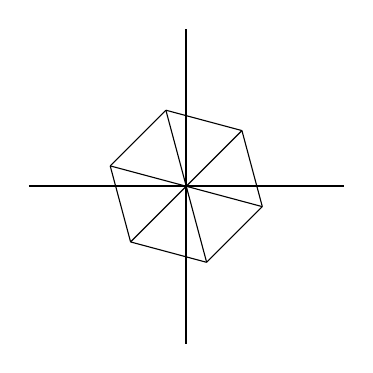
\begin{tikzpicture}
%\draw [help lines,black!20!white] (-1,-1) grid (4,4);

\draw[thick] (0,-2) -- (0,2);
\draw[thick] (-2,0) -- (2,0);

\foreach \x in {0,1,...,5}{
	\draw (0,0) -- ({cos(45 + 60*\x)},{sin(45 + 60*\x)});
	\draw ({cos(45 + 60*\x)},{sin(45 + 60*\x)}) -- ({cos(105 + 60*\x)},{sin(105 + 60*\x)});}



\end{tikzpicture}
\end{center}

And this is true in general. If $w\ne 0$ and $n\ge 3$, then the roots of $z^n = w$ form a regular $n$-gon.

\end{itemize}

I made a small note in the preceeding discussion which I would like to expand upon. Namely, how to describe complex circles.

\begin{thmbo}{}{rootsCircle}
The set of points $\{z\in\C| |z - z_0| = r\}$ is a circle of radius $r$ centered at $z_0$.
\end{thmbo}

\begin{proof} The circle of radius $r$ centered at $(x_0,y_0)$ in $\R^2$ is described by the equation $(x-x_0)^2 + (y-y_0)^2 = r^2$. We wish to show that $|z-z_0| = r$ is equivalent to this expression.

Suppose $z = x + iy$ and $z_0 = x_0 + iy_0$. Then:

$$r = |z-z_0| = |(x-x_0) + i(y-y_0)| = \sqrt{(x-x_0)^2 + (y-y_0)^2}$$

Squaring both sides gives the desired result.
\end{proof}

\section{Functions}

Our major goal is to talk about complex calculus: both differentiation and integration. To do so, we need some notion of a function. 

\begin{defbo}{Function}{function}\index{Function}\index{Function!domain}\index{Function!range}
Let $U,W$ be subsets of $\C$. A function $f:U\rightarrow W$ is a rule that assigns to each element $z\in U$ exactly one element $f(z) \in W$. $U$ is called the domain of $f$, and $W$ is called the codomain of $f$.

The range of $f$ is the set $\{f(z)|z\in U\}$. The range does not need to be all of $W$.
\end{defbo}

So, in essence, functions of a complex variable are defined exactly the same way any other function is. The difference here is that the domain and codomain both lie in planes, so we won't be able to draw graphs to visualize functions. After all, how do you visualize a 4-dimensional picture? Actually, we also aren't going to be able to use contour maps to understand these functions either

\begin{ex}{}{} Find the domain and range of the function $f(x + iy) = \frac{ix + y}{x - iy}$.

When finding the domain of a function given by a formula, take the largest set on which that formula makes sense. So, in this example, the formula gives an output whenever $x - iy\ne 0$. I.e., when $z\ne 0$. So, the domain of this function is $\C\setminus\{0\}$.

For the range, $w$ is in the range if there exists $z$ with $f(z) = w$. So, we have to solve the equation $\frac{ix + y}{x-iy} = w$.

There are two ways to do this, depending on whether you notice something.

\paragraph{Hard way:} Set $w = a+ib$. Then we want:
$$ix + y = (x-iy)(a+ib) = xa + yb + i(xb - ay)$$

So, $f(z) = w$ for some $z$ if there exist $x,y$ making this equation true.

If we look at the real and imaginary parts of this equation, we find that:
$$x = xb - ay$$
$$y = xa + yb$$

Alternatively, we can rewrite this as:
$$(b-1)x -ay = 0$$
$$ax +(b-1)y = 0$$

This is a system of linear equations in two variables, so we can solve this:
$$\amatrix{b-1&-a\\a&b-1}{0\\0}$$

Note, this matrix has determinant $(b-1)^2  + a^2$. If the determinant is non-zero, we have a unique solution $x = y = 0$. This would give $z = 0$, which is not in our domain. 

If the determinant is zero, then there is a non-trivial solution. So if $(b-1)^2 +a^2 = 0$, $w = a+ib$ is in the range. This occurs exactly when $a = 0$ and $b = 1$. I.e., when $w = i$.

\paragraph{Easy way:} Notice that $ix + y = i(x - iy)$. So, if $z\ne 0$, then $f(z) = i$. The range of $f$ is $\{i\}$.

\end{ex}

As this example illustrates, generally it is difficult to find the range of a complex function. But this isn't terribly different than working over the reals. Except for the very simple functions we see in first year calculus, it is also generally hard to find the range of a real function as well. Especially functions whose domain is in $\R^2$. The methods we used in this example do not generalize; finding ranges is always ad hoc.

Next, let's take a little tour of a few of the basic functions we're going to encounter. First, polynomials:

\begin{defbo}{Polynomials}{polynomial}\index{Polynomial}\index{Polynomial!degree} A polynomial $p$ on $\C$ is a function of the form:

$$p(z) = a_nz^n + \dots + a_1z + a_0 = \sum_{k = 0}^n a_kz^k$$

The degree of $p$ is the largest $n$ such that $a_n \ne 0$.
\end{defbo}

We're going to be spending a decent amount of time talking about polynomials in this course. Keep in mind that these don't behave the same way as real polynomials, and that we can have complex coefficients. $p(z) = z^2 + iz - (1-i)$ is a polynomial.

Let's also talk about root functions. Over the reals, it's fairly easy to define root functions: either $x$ has 0 $n$th roots, 1 $n$th root, or 2 $n$th roots. If it has no $n$th roots, then $f(x)$ isn't defined. If it has 1 $n$th root, then that's $f(x)$. And if it has 2 roots, then one is positive and we choose that to be $f(x)$.

This isn't possible over $\C$. We have $n$ $n$th roots, and we don't have any notion of positivity. (Notice, we've never talked about $z < w$ where $z,w$ are complex numbers. That's because it's not possible to define in a useful way.)

\begin{note}\index{Positive number}\index{<}
There is no notion of a positive complex number, and it does not mean anything to say that $z < w$ for complex numbers.

In this text, if we write $a < b$, it must be understood that $a,b$ are {\bf real numbers.}
\end{note}

So do we have an $n$th root function on $\C$? Let's start by taking a look at a bad way to define such a function:

\begin{ex}{}{} Consider the following (clearly false) proof:

\begin{claim} $1 = -1$.\end{claim}

\begin{proof} Let $z = re^{i\theta}$. Consider the function $f(z)$ defined by $f(z) = \sqrt{r}e^{i\frac{\theta}{2}}$. Note that $f(z)^2 = z$, and so $f(z)$ is a square root function.

As we have already seen, we can write $1 = e^{i0} = e^{i(2\pi)}$. Applying our function gives:


\begin{align*}f(1) &= f(e^{i0}) = \sqrt{1}e^{i\frac{0}{2}} = 1e^{i0} = 1\\
f(1) &= f(e^{i(2\pi)}) = \sqrt{1}e^{i\frac{2\pi}{2}} = e^{i\pi} = -1\end{align*}

Therefore, $1 = f(1) = -1$, as desired.\end{proof}


\exercisebox{ What's wrong with this argument?}

Well, if you take me at my word that $f(z)$ is a function, nothing. So that's the problem, $f(z)$ isn't a function. Not every formula defines a function, so we need to be careful.

In fact, our argument here really just shows that this formula doesn't define a function.

\end{ex}


So, if we want to define an $n$th root function, we need to be a lot more careful. The $n$th root is our first example of a common theme with complex formulae: it's a multivalued function.

\begin{defbo}{Multi-valued Function}{multifunc}\index{Function!multi-valued} A {\bf multi-valued function} $f$ on $\C$ is a rule that assigns to $z \in \C$ a set of (possibly more than one) outputs.

The output set of $f$ is still written as $f(z)$.
\end{defbo}

For example, the formula $f(re^{i\theta}) = \sqrt{r}e^{i\frac{\theta}{2}}$ is a rule that assigns to $z\ne 0$ its two square roots. It therefore defines a multi-valued function. We can similarly look at all $n^\text{th}$ roots as giving multi-valued function. The notation for this is:

\begin{defbo}{$z^{\frac{1}{n}}$}{multifuncroot}
For $z \in \C$, we define $z^{\frac{1}{n}} = \{w\in \C: w^n = z\}$. That is, $z^\frac{1}{n}$ is a mutli-valued function whose outputs are the $n$th roots of $z$.

Explicitly, if we write $z = re^{i\theta}$ for $z\ne 0$, then the formula $f(z) = \sqrt[n]{r}e^{i\frac{\theta}{n}}$ gives $z^\frac{1}{n}$. If we collect all outputs $f(z)$ given by taking different arguments of $z$, we get:

$$z^\frac{1}{n} = \left\{\sqrt[n]{|z|}e^\frac{i\theta}{n}: \theta\in\arg(z)\right\}$$

\end{defbo}


We need to be careful now. Our goal is to do calculus. That's going to require us to have functions to work with. So how can we go from having a multi-valued function to an actual function?

\begin{defbo}{Branch of a Multi-valued Function}{branch}\index{Function!branch} \index{Branch}
Let $f$ be a multivalued function with domain $U$. A {\bf branch} of $f$ is a function $g:U\rightarrow \C$ such that $g(z) \in f(z)$. (Remember that $f(z)$ is a set, so this makes sense.)
\end{defbo}

So, for each input, we pick one output (out of the possible outputs given by the multi-valued function) to be the output of the branch. Now, without care, you can choose some truely bizarre branches. For example, for the square root, we could say that if $z = x + iy$, we choose the square root $a+ bi$ with $a \ge 0$ if $x$ is rational, and if $x$ is irrational we choose the square root with $a < 0$.

This is a contrived example, but that's the point. You can cook up some truly weird and unpleasant branches if you set your mind to it. Is there some way to choose our branches nicely? For some nice functions yes, and it comes down to the argument of $z$, actually.

\begin{ex}{}{}\index{$\arg(z)$}\index{Argument!$\arg(z)$} Let $z\in \C$. For $z\ne 0$, we define $\arg(z) = \{\theta\in \R| z = |z|e^{i\theta}\}$ (i.e., $\arg(z)$ is the set of all arguments of $z$). Then this is a multi-valued function (in fact, infinitely-valued) function on $\C$.

One way to take branches of $\arg$ is to specify a range of angles. So, for example, we could get a branch of the argument $\arg_0(z)$ by choosing $\arg_0(z) = \theta$ where $\theta$ is the unique angle in $\arg(z) \cap [0,2\pi)$. This rule assigns to each $z\ne 0$ a single argument.
\end{ex}

\begin{ex}{}{} Let $\theta \in \R$. Define $\arg_0(z)$ to be the branch of $\arg(z)$ with $\arg_0(z)\in [\theta, \theta + 2\pi)$.

Then for $z = re^{i\theta}$, we can define $z^{\frac{1}{2}} = \sqrt{r}e^{i\frac{\arg_0(z)}{2}}$. This gives a branch of the square root.

Notice that $(z^{\frac{1}{2}})^2 = \sqrt{r}^2(e^{i\frac{\arg_0(z)}{2}})^2 = re^{i\frac{2\arg_0(z)}{2}} = re^{i\arg_0(z)} = z$. So this is actually a square root.

It also only gives one output to each input. Each $z\in \C$, except $z = 0$, has a unique argument $\arg_0(z)$ between $\theta$ and $\theta + 2\pi$. As such, the formula doesn't depend on the angle we choose for $z$. Indeed, there is no choice!
\end{ex}

This may seem a bit arcane. Frankly, this is one of the more difficult concepts in this course. We're going to come back to it once we introduce the complex logarithm (which will also be a multi-valued function). I wanted to introduce the concept before we run into that.

\paragraph{Notation:} Very often, we will write equations involving multi-valued functions. For example, we can write the quadratic formula as:

$$z = \frac{-b+ (b^2 - 4ac)^\frac{1}{2}}{2a}$$

It is important to understand that we are saying that $z$ takes on two different values, one for each different value of the square root.


\subsection{The Exponential Function}

In definition \ref{def:eulerForm}, we defined $e^{i\theta}$ for any $\theta \in \C$. We can use this to give a definition of $e^z$.

\begin{defbo}{The Exponential Function}{exponential}\index{Exponential function} 
Let $z = x + iy$. Then we define the exponential $e^z$ as:

$$e^z = e^xe^{iy} = e^x(\cos(y) + i\sin(y))$$
\end{defbo}

Unlike roots, this is a function. Indeed, for each $z\in \C$, there is a unique choice of $x,y\in \R$ such that $z = x+iy$, and so we don't get multiple values coming from this formula.

Is this a good definition? What might we expect to be true of a complex exponential function. We would like:

\begin{itemize}
\item $e^ze^w = e^{z + w}$
\item $e^z \ne 0$
\item For $z = r\in R$, we would like $e^z$ (the complex exponential) to be equal to $e^r$ (the real exponential).
\item If $z = iy$, we should have that $e^z = \cos(y) + i\sin(y)$, so that this formula also agrees with Euler's formula.
\item It should be a differentiable function, once we've defined what that means in $\C$.

\end{itemize}


And these turn out to all be true! The third and fourth are a quick exercise in using the definition. We'll prove the first very quickly:

\begin{proof} Let $z = x + iy$ and $w = a + ib$. Then:

\begin{align*} e^ze^w &= e^xe^{iy}e^ae^{ib} \\
&= e^xe^ae^{i(y+b)} \qquad \qquad (\text{ by theorem }\ref{thm:polarmult})\\
&= e^{x+a}e^{i(y+b)}\end{align*}

This is exactly $e^{z + w}$ since $z + w = (x+a) + i(y+b)$.\end{proof}


\begin{ex}{}{} Let's compute a few exponentials. Find $e^{1 + i}$ and $e^{1-i}$.

Well, we compute:

$$e^{1 + i} = e^1e^{i} = e^1(\cos(1) + i\sin(1)$$
$$e^{1 - i} = e^1e^{-i} = e^1(\cos(-1) + i\sin(-1) = e^1(\cos(1) - i\sin(1))$$

\end{ex}

Did you notice anything about these two numbers? Give a conjecture for the relationship between $e^z$ and $e^{\OL{z}}$.

\begin{ex}{}{}A function $f$ is called {\bf injective} if $f(z) = f(w)$ implies $z = w$.

\exercisebox{True or false: $f(z) = e^z$ is an injective function.}

False. We have already seen that $e^{0} = e^{i2\pi}$. In fact, for any $w\ne 0$, $e^z =w$ has infinitely many solutions!
\end{ex}


\begin{ex}{}{} Let $w = 1 + 4i$. Solve the equation $e^z = w$.

Let $z = x + iy$. Then $e^xe^{iy} = 1+ 4i$. This tells us that:
$$e^x = |w| = \sqrt{17}$$

So we conclude that $x = \ln(\sqrt{17})$.

Further, the expression $w = e^xe^{iy}$ tells us that $y$ is an argument for $w$! So, we need to find the arguments for $w$. We see that $w = \sqrt{17}e^{i\arctan(4)}$.

Therefore, $z = \ln(\sqrt{17}) + i\arctan(4)$.

\exercisebox{There is an error in this argument. What is it?}

 We know that $y$ is AN argument for $w$. Not that $y$ is this particular argument for $w$. Instead, we can only conclude that $y = \arctan(4) + 2k\pi$ for some $k\in \Z$, and therefore $z = \ln(\sqrt{17}) + i(\arctan(4) + 2k\pi)$.
\end{ex}

\begin{note} $\ln(\sqrt{17}) + i\arctan(4)$ and $\ln(\sqrt{17}) + i(\arctan(4) + 2\pi)$ are different complex numbers! While $\arctan(4)$ and $\arctan(4) + 2\pi$ point in the same direction as angles, $y$ is not an angle. $y$ is the vertical component of the complex number $z$.

This distinction is important. $y$ is not an angle, and so we can't ignore this $2k\pi$.\end{note}

\begin{ex}{}{hardexpo} Solve the equation $e^{iz} - e^{-iz} = 2i$.

It is possible to solve this equation by setting $z = x+ iy$, expanding into rectangular form, and then solving the resulting equations. However, this turns out to be fairly difficult.

Instead, let $e^{iz} = w$. Then we have:
$$w - \frac{1}{w} = 2i$$

After some quick algebra, we can rearrange this to become:
$$w^2 - 2iw - 1 = 0$$

Now, from your homework, we know that we can solve this using the quadratic formula:
$$w = \frac{2i \pm (-4 + 4)^{\frac{1}{2}}}{2} = i$$

So, the solutions $z$ to the original equation satisfy $e^{iz} = i$. Let $z = x+iy$. Then $e^{-y + ix} = i$. This gives $e^{-y} = 1$, so $y = 0$.

Also, we know that $x$ is an argument for $i$, so $x = \frac{\pi}{2} + 2k\pi$ for $k\in \Z$. Therefore, $e^{iz} - e^{-iz} = 2i$ if and only if $z = \frac{\pi}{2} + 2k\pi$ for some $k\in \Z$.

\end{ex}


\begin{ex}{}{} True or false: For any $z\in \C$, $e^z > 0$.

False. Remember, it is nonsense to say that $a > b$ if $a,b$ are complex numbers. $e^z$ can be any complex number (except for $0$), so this is a nonsense statement.

More concretely, $e^{i\pi} = -1 \not> 0$.

\end{ex}

\subsection{Complex Trigonometric Functions}

Looking at Euler's formula, $e^{i\theta} = \cos(\theta) + i\sin(\theta)$, it seems like there's a connection between trigonometric functions and the complex exponential.

If we play around with this fact, we can see:
\begin{align*}
e^{i\theta} &= \cos(\theta) + i\sin(\theta)\\
e^{-i\theta} &= \cos(-\theta) + i\sin(-\theta) = \cos(\theta) - i\sin(\theta)
\end{align*}

Adding these expressions together, we see that:
$$\cos(\theta) = \frac{e^{i\theta} + e^{-i\theta}}{2}$$
$$\sin(\theta) = \frac{e^{i\theta} - e^{-i\theta}}{2i}$$

Since this is our only connection between trigonometric functions and complex numbers, it seems reasonable to use this to define complex versions of $\cos(z)$ and $\sin(z)$.

\begin{defbo}{Trigonometric Functions}{trigFunc}\index{Function!trigonometric} The complex trigonometric functions $\cos(z)$ and $\sin(z)$ are defined by:
$$\cos(z) = \frac{e^{iz} + e^{-iz}}{2}$$
$$\sin(z) = \frac{e^{iz} - e^{-iz}}{2i}$$

The other trigonometric functions $\tan(z)$, $\sec(z)$, $\csc(z)$, and $\cot(z)$ are defined exactly how you would expect.
\end{defbo}

Just like for our complex exponential, notice that if $z = x\in \R$, then $\cos(z)$ is exactly the real cosine function $\cos(x)$, and similarly for $\sin(z)$. So this isn't totally unreasonable.


Many of the usual properties of the real trigonometric functions are still satisfied by these complex functions as well. For example:

\begin{ex}{}{} We know that the real function $\cos(x)$ is $2\pi$ periodic. I.e., $\cos(x) = \cos(x + 2\pi)$. This is still true over $\C$.

To see this, note that:
$$\cos(z + 2\pi) = \frac{e^{i(z + 2\pi)} + e^{-i(z + 2\pi)}}{2} = \frac{e^{iz}e^{i2\pi} + e^{-iz}e^{-i2\pi}}{2} = \frac{e^{iz} + e^{-iz}}{2} = \cos(z)$$
\end{ex}

However, these complex functions can have some wildly different behavior as well.

\begin{ex}{}{} True or false: $-1 \le |\sin(z)| \le 1$ for any $z\in \C$.

As we saw in class, when looking at $\sin(iy)$, we see that for $y$ very large, $|\sin(iy)|$ is very large. In fact, $|\sin(iy)| \approx \frac{e^{|y|}}{2}$.

In fact, the range of $\sin(z)$ is actually $\C$!

\end{ex}

\begin{ex}{}{} Find all solutions to $\sin(z) = 1$.

We are looking for all $z$ for which $\sin(z) = \frac{e^{iz} - e^{-iz}}{2i} = 2i$. Notice that this is equivalent to solving $e^{iz} - e^{-iz} = 1$. As we saw in example \ref{exa:hardexpo}, the solutions to this are precisely $z = \frac{\pi}{2} + 2k\pi$ for $k\in \Z$. So the only solutions to $\sin(z) = 1$ are real solutions.

\end{ex}

\subsection{The Complex Logarithm}

We have a notion of complex exponentiation. Do we have a corresponding notion of complex logarithms?

To begin, what is a logarithm? What does it mean to say that $w$ is a logarithm for $z$?

\begin{defbo}{Logarithms}{logarithm}\index{Logarithm} 
Let $z\in \C$. We say that $w$ is a logarithm for $z$ if $e^w = z$.
\end{defbo}

We've already seen an example of finding a logarithm. Last class, we showed that the solutions to $e^{z} = 1 + 4i$ are of them form $z = \ln(\sqrt{17}) + i(\arctan(4) + 2k\pi)$ for $k\in \Z$. So, $1 + 4i$ has many logarithms. These are precisely the $z$ listed above.


Is there a general formula for finding the logarithms of $z\in \C$, or do we need to do it by hand each time we wish to solve $e^z = w$?

\begin{thmbo}{Calculating Logarithms}{logCalc}
 Let $z = re^{i\theta}$ with $z\ne 0$. Then the logarithms of $z$ are the complex numbers $\ln(r) + i(\theta + 2k\pi)$, where $k\in \Z$. Put another way, $\log(z) = \ln|z| + i\arg(z)$, remembering that we mean this as multi-valued functions.


If $z = 0$, then $z$ has no logarithms.
\end{thmbo}

\begin{proof} First, we handle the situation where $z\ne 0$. Suppose $w = a +bi$ and $e^w = z$. Then:
$$e^ae^{ib} = re^{i\theta}$$

Taking the modulus of both sides, we see that $e^a = r$, and so $a = \ln(r)$, which is defined since $r\ne 0$.

Now, we can see that $re^{ib} = z$, and so $b$ is an argument for $z$. As we have shown before, this means that $b = \theta + 2k\pi$ for some $k\in Z$.

As for $z = 0$, notice that $|e^w| = e^a \ne 0$. However, $|z| = 0$. So, we cannot have $e^w = z$.

\end{proof}

The complex logarithm is the most important example of a multi-valued function. In fact, all of the examples we are going to see in this course (including the ones we already have seen!) will depend on the complex logarithm.

\begin{notation} We are often very lazy with our notation for logarithms. If $e^w = z$, we very often write that $w = \log(z)$.

But, as we've seen, it is possible to have $w_1\ne w_2$ with $e^{w_1} = e^{w_2} = z$. So is $w_1 = \log(z)$ or is $w_2 = \log(z)$?

The answer is that $\log(z)$ isn't really one number. The complex logarithm is a multi-valued function, and so $w_1$ and $w_2$ are two different values of the same multi-valued function. So when we say that $w = \log(z)$, we really mean that $w$ is {\bf one of} the logarithms of $z$.
\end{notation}

\begin{defbo}{$\log(z)$}{log}\index{Function!$\log(z)$}
The complex logarithm $\log(z)$ is the multi-valued function:
$$\log(z) = \{w\in \C| e^w = z\}$$

For any $z\ne 0$, $\log(z)$ is infinitely-valued.
\end{defbo}


\begin{ex}{}{} Suppose we know that $\log(z) = 1 + 3i$. Is it possible that $\log(z) = 1 + 7i$?

No. We would need $e^{1 + 3i} = e^{1 + 7i}$. But these have different angular components. The angles $3$ and $7$ do not point in the same direction!
\end{ex}



\begin{defbo}{Complex Exponentiation}{exponentiation}\index{$z^a$} 
Let $a,z\in \C$. Then $z^a = e^{a\log(z)}$.
\end{defbo}

How do we interpret this? After all, we just discussed that $\log(z)$ isn't one number. This formula should be interpretted as saying that $z^a$ is a multi-valued function, and that its values are $e^{aw}$ where $w$ is a logarithm for $z$.


\begin{ex}{}{} This definition has some surprising consequences. For example, every value of $i^i$ is real!

Why is that? Well, $i^i = e^{i\log(i)}$. However, since $|i| = 1$, we see that the logarithms of $i$ are:
$$\log(i) = \ln(1) + i\left(\frac{\pi}{2} + 2k\pi\right) = i\left(\frac{\pi}{2} + 2k\pi\right)$$

As such, $i^i = e^{i^2\left(\frac{\pi}{2} + 2k\pi\right)} = e^{-\frac{\pi}{2} + 2k\pi}$, which is a real number!\end{ex}

\begin{ex}{}{}Consider the following claim:

\begin{fthmbo}{}{ex1} Every complex number is real.\end{fthmbo}

You should quickly convince yourself that this is false. For example, why is $i$ not real? (What property defines $i$?)

So, if this is a false claim, any proof of this claim must have an error. Find the error (or errors, if there are more than one) in the following proof.

\MyCBox{black}{white}{\begin{proof} Let $z\in \C$, and write $z$ in polar form as $z = re^{i\theta}$. Then we find that:
$$z = re^{i\theta} = re^{i\left(\frac{2\pi\theta}{2\pi}\right)} = r(e^{2\pi i})^{\frac{\theta}{2\pi}}$$

But $e^{2\pi i} = \cos(2\pi) + i\sin(2\pi) = 1$. So:
$$z = r(1^{\frac{\theta}{2\pi}}) = r \in \R$$

Since $z \in \R$ for any complex number $z$, every complex number is real.

\end{proof}}

Be careful. Any errors are subtle. If you think you have an easy answer, chances are your answer is not correct.

\paragraph{Solution:} As we discussed in class, the error occurs in two places. When we write:
$$e^{i\frac{2\pi\theta}{2\pi}} = (e^{i2\pi})^{\frac{\theta}{2\pi}}$$


\noin we are choosing a branch $f(z)$ of the multivalued function $z^{\frac{\theta}{2\pi}}$ so that $f(1) = e^{i\theta}$.

On the other hand, when we say that $1^{\frac{\theta}{2\pi}} = 1$, we are choosing a branch $g(z)$ with $g(1) = 1$. We're working with two different branches as if they are the same!
\end{ex}

Now that we have talked about how they are multivalued, and how that requires some care, let's talk about their branches. Corresponding to the principal Argument $\Arg(z)$, there is a principal branch of these multivalued functions as well:

\begin{defbo}{Principal Logarithm}{prinLog}\index{Logarithm!principal}
Let $z\in \C\setminus(-\infty,0]$. The principal logarithm of $z$ is:
$$\Log(z) = \ln|z| + i\Arg(z)$$
\end{defbo}

\begin{defbo}{Principal Branch of $z^a$}{prinpower}\index{$z^a$!principal branch}
The principal branch of $z^a$ is given by $e^{a\Log(z)}$.
\end{defbo}

\begin{ex}{}{} Find the principal value of $i^{1 - i}$.

The principal value (which comes from the principal branch) is:
$$e^{(1-i)\Log(i)} = e^{(1-i)i\frac{\pi}{2}} = e^{\frac{\pi}{2} + i\frac{\pi}{2}} = e^{\frac{\pi}{2}}i$$
\end{ex}

\begin{ex}{}{} Let $n\in \Z$. Is $z^n$ a single valued function?

Well, $z^n = e^{n\log(z)}$. Let $z = re^{i\theta}$. Then:
$$z^n = e^{n\log(z)} = e^{n(\ln|z| + i(\theta + 2k\pi))}$$

\noin where $k\in \Z$. However, notice that $nk\in \Z$, so $e^{i(2nk)\pi} = 1$. Therefore:
$$z^n = e^{n(\ln|z| + i\theta)} = e^{\ln(|z|^n) + in\theta} = |z|^ne^{in\theta}$$

So this is a single valued function. Regardless of our choice of argument, we get the same result.
\end{ex}

\begin{ex}{}{} Consider the formula $f(z) = a^z$. Is this a function?

Let $z = x +iy$. We have $a^z = e^{z\log(a)} = e^{z(\ln|a| + i\arg(a))} = e^{(x\ln|a| - y\arg(a)) + i(x\arg(a) + y\ln|a|)}$. This formula outputs a single value if and only if $e^{y\arg(a) - ix\arg(a)}$ doesn't depend on the choice of argument.

Notice that if $y\ne 0$, then different arguments for $a$ give different moduli for $a^z$, so we must have $y = 0$. However, if $y = 0$, then $|e^{y\arg(a) - ix\arg(a)}| = 1$. Also, the angular component of $e^{y\arg(a) - ix\arg(a)}$ must not depend on the choice of argument for $a$. Suppose $a = re^{i\theta}$ for some $\theta$. Then $\theta$ and $\theta + 2\pi$ are both arguments for $a$. As such, we need that $e^{ix\theta} = e^{ix(\theta + 2\pi)}$. This gives us that $e^{i2\pi x} = 1$, so $x\in \Z$. The converse is also true, if $x\in \Z$, then $e^{ix\arg(a)}$ does not depend on the choice of argument.
\end{ex}

So, this tells us that $a^z$ is a multi-valued function as well! Does that mean that $e^z$ is multi-valued? The answer to that is no. Our definition of $e^z$ doesn't depend on the argument of $e$. Technically, our definition of $e^z$ is the principal branch of the function:
$$f(z) = e^{\RE(z\log(e))}(\cos(\IM(z\log(e))) + i\sin(\IM(z\log(e))))$$

However, to avoid unnecessary notational baggage (after all, this function is a bit of a mouthful) and to avoid unnecessary abstraction, $e^z$ will always be understood to be an exception to $a^z$ being a multi-valued function.

\begin{ex}{}{} Find the range of $\sin(z)$.

Let $w\in \C$. We would like to see if there exists some $z\in\C$ with $\sin(z) = w$. Supposing there is, we have:
$$\frac{e^{iz} - e^{-iz}}{2i} = w$$

Rearranging gives $e^{iz} - 2iw - e^{-iz} = 0$. Let $u = e^{iz}$. Since $u\ne 0$, we see that:
$$u - 2iw - \frac{1}{u} = 0 \iff u^2 - 2iwu - 1 = 0$$

And the quadratic formula tells us that:
$$u = iw + (-w^2 + 1)^{\frac{1}{2}}$$

And so $z = \frac{\log(u)}{i}$.

But wait, we're not done! We need to know that $\log(u)$ actually exists for any given $w$. We assumed $u\ne 0$, but are we guaranteed that it is? After all, it depends on $w$. How do we know there doesn't exist some $w$ such that $u = 0$?

Suppose $u = 0$. Then $(1 - w^2)^{\frac{1}{2}} = iw$. Squaring both sides gives $1 - w^2 = -w^2$, which cannot occur. So $u\ne 0$, and therefore such a $z$ exists for any $w$.
\end{ex}

This example gives us an idea of how to define inverse trig functions as well:

\begin{defbo}{$\arcsin$}{arcsin}\index{Function!$\arcsin$} Let $z\in \C$. Then:

$$\arcsin(z) = -i\log(iz + (1 - z^2)^{\frac{1}{2}})$$

Further, the principal arcsin is given by:
$$\Arcsin(z) = -i\Log(iz + (1-z^2)^{\frac{1}{2}})$$

\noin where $(1 - z^2)^{\frac{1}{2}}$ is the principal square root.
\end{defbo}
